\chapter{Peliteoria}

Tässä luvussa keskitymme kahden pelaajan peleihin,
joissa molemmat pelaajat tekevät
samanlaisia siirtoja eikä pelissä ole satunnaisuutta.
Tavoitteemme on etsiä strategia, jota käyttäen
pelaaja pystyy voittamaan pelin toisen pelaajan
toimista riippumatta, jos tämä on mahdollista.

Osoittautuu, että kaikki tällaiset pelit ovat
pohjimmiltaan samanlaisia ja niiden analyysi on
mahdollista \key{nim-teorian} avulla.
Perehdymme aluksi yksinkertaisiin tikkupeleihin,
joissa pelaajat poistavat tikkuja kasoista,
ja yleistämme sitten näiden pelien teorian kaikkiin peleihin.

\section{Pelin tilat}

Tarkastellaan peliä, jossa kasassa on $n$ tikkua.
Pelaajat $A$ ja $B$ siirtävät vuorotellen ja
pelaaja $A$ aloittaa.
Jokaisella siirrolla pelaajan tulee poistaa
1, 2 tai 3 tikkua kasasta.
Pelin voittaa se pelaaja, joka poistaa viimeisen tikun.

Esimerkiksi jos $n=10$, peli saattaa edetä seuraavasti:
\begin{enumerate}[noitemsep]
\item Pelaaja $A$ poistaa 2 tikkua (jäljellä 8 tikkua).
\item Pelaaja $B$ poistaa 3 tikkua (jäljellä 5 tikkua).
\item Pelaaja $A$ poistaa 1 tikun (jäljellä 4 tikkua).
\item Pelaaja $B$ poistaa 2 tikkua (jäljellä 2 tikkua).
\item Pelaaja $A$ poistaa 2 tikkua ja voittaa.
\end{enumerate}
Tämä peli muodostuu tiloista $0,1,2,\ldots,n$,
missä tilan numero vastaa sitä, montako tikkua
kasassa on jäljellä.
Tietyssä tilassa olevan pelaajan valittavana on,
montako tikkua hän poistaa kasasta.

\subsubsection{Voittotila ja häviötila}

\index{voittotila}
\index{häviötila}

\key{Voittotila} on tila, jossa oleva pelaaja voittaa
pelin varmasti, jos hän pelaa optimaalisesti.
Vastaavasti \key{häviötila} on tila,
jossa oleva pelaaja häviää varmasti, jos vastustaja
pelaa optimaalisesti.
Osoittautuu, että pelin tilat on mahdollista luokitella
niin, että jokainen tila on joko voittotila tai häviötila.

Yllä olevassa pelissä tila 0 on selkeästi häviötila,
koska siinä oleva pelaaja häviää pelin suoraan.
Tilat 1, 2 ja 3 taas ovat voittotiloja,
koska niissä oleva pelaaja voi poistaa
1, 2 tai 3 tikkua ja voittaa pelin.
Vastaavasti tila 4 on häviötila, koska mikä tahansa
siirto johtaa toisen pelaajan voittoon.

Yleisemmin voidaan havaita, että jos tilasta on
jokin häviötilaan johtava siirto, niin tila on voittotila,
ja muussa tapauksessa tila on häviötila.
Tämän ansiosta voidaan luokitella kaikki pelin tilat
alkaen varmoista häviötiloista, joista ei ole siirtoja
mihinkään muuhun tilaan.

Seuraavassa on pelin tilojen $0 \ldots 15$ luokittelu
($V$ tarkoittaa voittotilaa ja $H$ tarkoittaa häviötilaa):
\begin{center}
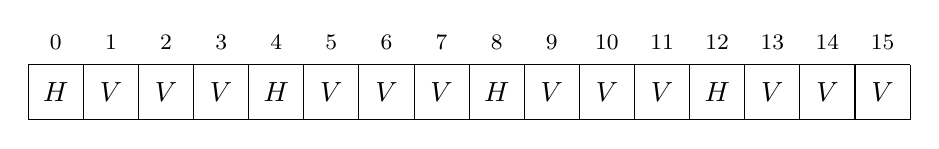
\begin{tikzpicture}[scale=0.7]
\draw (0,0) grid (16,1);

\node at (0.5,0.5) {$H$};
\node at (1.5,0.5) {$V$};
\node at (2.5,0.5) {$V$};
\node at (3.5,0.5) {$V$};
\node at (4.5,0.5) {$H$};
\node at (5.5,0.5) {$V$};
\node at (6.5,0.5) {$V$};
\node at (7.5,0.5) {$V$};
\node at (8.5,0.5) {$H$};
\node at (9.5,0.5) {$V$};
\node at (10.5,0.5) {$V$};
\node at (11.5,0.5) {$V$};
\node at (12.5,0.5) {$H$};
\node at (13.5,0.5) {$V$};
\node at (14.5,0.5) {$V$};
\node at (15.5,0.5) {$V$};

\footnotesize
\node at (0.5,1.4) {$0$};
\node at (1.5,1.4) {$1$};
\node at (2.5,1.4) {$2$};
\node at (3.5,1.4) {$3$};
\node at (4.5,1.4) {$4$};
\node at (5.5,1.4) {$5$};
\node at (6.5,1.4) {$6$};
\node at (7.5,1.4) {$7$};
\node at (8.5,1.4) {$8$};
\node at (9.5,1.4) {$9$};
\node at (10.5,1.4) {$10$};
\node at (11.5,1.4) {$11$};
\node at (12.5,1.4) {$12$};
\node at (13.5,1.4) {$13$};
\node at (14.5,1.4) {$14$};
\node at (15.5,1.4) {$15$};
\end{tikzpicture}
\end{center}

Tämän pelin analyysi on yksinkertainen:
tila $k$ on häviötila, jos $k$ on jaollinen 4:llä,
ja muuten tila $k$ on voittotila.
Optimaalinen tapa pelata peliä on
valita aina sellainen siirto, että vastustajalle
jää 4:llä jaollinen määrä tikkuja,
kunnes lopulta tikut loppuvat ja vastustaja on hävinnyt.

Tämä pelitapa edellyttää luonnollisesti sitä,
että tikkujen määrä omalla siirrolla ei ole
4:llä jaollinen. Jos näin kuitenkin on, mitään ei ole
tehtävissä vaan vastustaja voittaa
pelin varmasti, jos hän pelaa optimaalisesti.

\subsubsection{Tilaverkko}

Tarkastellaan sitten toisenlaista tikkupeliä,
jossa tilassa $k$ saa poistaa minkä tahansa
määrän tikkuja $x$, kunhan $k$ on jaollinen $x$:llä
ja $x$ on pienempi kuin $k$.
Esimerkiksi tilassa 8 on sallittua poistaa
1, 2 tai 4 tikkua, mutta tilassa 7
ainoa mahdollinen siirto on poistaa 1 tikku.

Esitetään pelin tilat $1 \ldots 9$ \key{tilaverkkona}, jossa solmut ovat pelin tiloja
ja kaaret kuvaavat mahdollisia siirtoja tilojen välillä:

\begin{center}
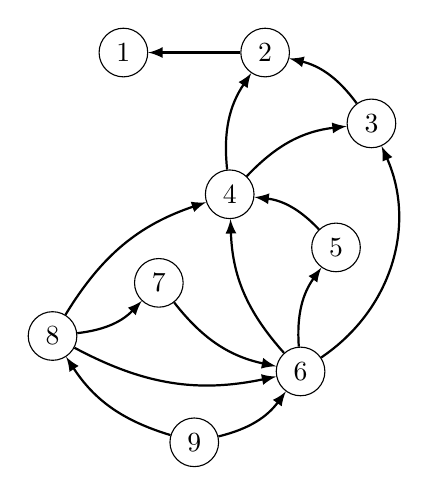
\begin{tikzpicture}[scale=0.9]
\node[draw, circle] (1) at (0,0) {$1$};
\node[draw, circle] (2) at (2,0) {$2$};
\node[draw, circle] (3) at (3.5,-1) {$3$};
\node[draw, circle] (4) at (1.5,-2) {$4$};
\node[draw, circle] (5) at (3,-2.75) {$5$};
\node[draw, circle] (6) at (2.5,-4.5) {$6$};
\node[draw, circle] (7) at (0.5,-3.25) {$7$};
\node[draw, circle] (8) at (-1,-4) {$8$};
\node[draw, circle] (9) at (1,-5.5) {$9$};

\path[draw,thick,->,>=latex] (2) -- (1);
\path[draw,thick,->,>=latex] (3) edge [bend right=20] (2);
\path[draw,thick,->,>=latex] (4) edge [bend left=20] (2);
\path[draw,thick,->,>=latex] (4) edge [bend left=20] (3);
\path[draw,thick,->,>=latex] (5) edge [bend right=20] (4);
\path[draw,thick,->,>=latex] (6) edge [bend left=20] (5);
\path[draw,thick,->,>=latex] (6) edge [bend left=20] (4);
\path[draw,thick,->,>=latex] (6) edge [bend right=40] (3);
\path[draw,thick,->,>=latex] (7) edge [bend right=20] (6);
\path[draw,thick,->,>=latex] (8) edge [bend right=20] (7);
\path[draw,thick,->,>=latex] (8) edge [bend right=20] (6);
\path[draw,thick,->,>=latex] (8) edge [bend left=20] (4);
\path[draw,thick,->,>=latex] (9) edge [bend left=20] (8);
\path[draw,thick,->,>=latex] (9) edge [bend right=20] (6);
\end{tikzpicture}
\end{center}

Tämä peli päättyy aina tilaan 1, joka on häviötila,
koska siinä ei voi tehdä mitään siirtoja.
Pelin tilojen $1 \ldots 9$ luokittelu on seuraava:

\begin{center}
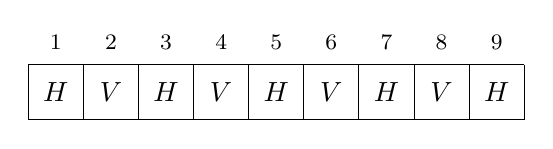
\begin{tikzpicture}[scale=0.7]
\draw (1,0) grid (10,1);

\node at (1.5,0.5) {$H$};
\node at (2.5,0.5) {$V$};
\node at (3.5,0.5) {$H$};
\node at (4.5,0.5) {$V$};
\node at (5.5,0.5) {$H$};
\node at (6.5,0.5) {$V$};
\node at (7.5,0.5) {$H$};
\node at (8.5,0.5) {$V$};
\node at (9.5,0.5) {$H$};

\footnotesize
\node at (1.5,1.4) {$1$};
\node at (2.5,1.4) {$2$};
\node at (3.5,1.4) {$3$};
\node at (4.5,1.4) {$4$};
\node at (5.5,1.4) {$5$};
\node at (6.5,1.4) {$6$};
\node at (7.5,1.4) {$7$};
\node at (8.5,1.4) {$8$};
\node at (9.5,1.4) {$9$};
\end{tikzpicture}
\end{center}

Yllättävää kyllä, tässä pelissä kaikki
parilliset tilat ovat voittotiloja ja
kaikki parittomat tilat ovat häviötiloja.

\section{Nim-peli}

\index{nim-peli}

\key{Nim-peli} on yksinkertainen peli,
joka on tärkeässä asemassa peliteoriassa,
koska monia pelejä voi pelata samalla
strategialla kuin nim-peliä.
Tutustumme aluksi nim-peliin ja yleistämme
strategian sitten muihin peleihin.

Nim-pelissä on $n$ kasaa tikkuja,
joista kussakin on tietty määrä tikkuja.
Pelaajat poistavat kasoista tikkuja vuorotellen.
Joka vuorolla pelaaja valitsee yhden kasan,
jossa on vielä tikkuja,
ja poistaa siitä minkä tahansa määrän tikkuja.
Pelin voittaa se, joka poistaa viimeisen tikun.

Nim-pelin tila on muotoa $[x_1,x_2,\ldots,x_n]$,
jossa $x_k$ on tikkujen määrä kasassa $k$.
Esimerkiksi $(10,12,5)$ tarkoittaa peliä,
jossa on kolme kasaa ja tikkujen määrät ovat 10, 12 ja 5.
Tila $(0,0,\ldots,0)$ on häviötila,
koska siitä ei voi poistaa mitään tikkua,
ja peli päättyy aina tähän tilaan.

\subsubsection{Analyysi}
\index{nim-summa}
Osoittautuu, että nim-pelin tilan luonteen
kertoo \key{nim-summa} $x_1 \oplus x_2 \oplus \cdots \oplus x_n$,
missä $\oplus$ tarkoittaa xor-operaatiota.
Jos nim-summa on 0, tila on häviötila,
ja muussa tapauksessa tila on voittotila.
Esimerkiksi tilan $(10,12,5)$ nim-summa on
$10 \oplus 12 \oplus 5 = 3$, joten tila on voittotila.

Mutta miten nim-summa liittyy nim-peliin?
Tämä selviää tutkimalla, miten nim-summa muuttuu,
kun nim-pelin tila muuttuu.

~\\
\noindent
\textit{Häviötilat:}
Pelin päätöstila $[0,0,\ldots,0]$ on häviötila,
ja sen nim-summa on 0, kuten kuuluukin.
Muissa häviötiloissa mikä tahansa siirto johtaa
voittotilaan, koska yksi luvuista $x_k$ muuttuu
ja samalla pelin nim-summa muuttuu
eli siirron jälkeen nim-summasta tulee jokin muu kuin 0.

~\\
\noindent
\textit{Voittotilat:}
Voittotilasta pääsee häviötilaan muuttamalla
jonkin kasan $k$ tikkujen määräksi $x_k \oplus s$,
missä $s$ on pelin nim-summa.
Vaatimuksena on, että $x_k \oplus s < x_k$,
koska kasasta voi vain poistaa tikkuja.
Sopiva kasa $x_k$ on sellainen,
jossa on ykkösbitti samassa kohdassa kuin
$s$:n vasemmanpuoleisin ykkösbitti.

~\\
\noindent
Tarkastellaan esimerkkinä tilaa $(10,2,5)$.
Tämä tila on voittotila,
koska sen nim-summa on 3.
Täytyy siis olla olemassa siirto,
jolla tilasta pääsee häviötilaan.
Selvitetään se seuraavaksi.

\begin{samepage}
\noindent
Pelin nim-summa muodostuu seuraavasti:

\begin{center}
\begin{tabular}{r|r}
10 & \texttt{1010} \\
12 & \texttt{1100} \\
5 & \texttt{0101} \\
\hline
3 & \texttt{0011} \\
\end{tabular}
\end{center}
\end{samepage}

Tässä tapauksessa
10 tikun kasa on ainoa,
jonka bittiesityksessä on ykkösbitti
samassa kohdassa kuin 
nim-summan vasemmanpuoleisin ykkösbitti:

\begin{center}
\begin{tabular}{r|r}
10 & \texttt{10\textcircled{1}0} \\
12 & \texttt{1100} \\
5 & \texttt{0101} \\
\hline
3 & \texttt{00\textcircled{1}1} \\
\end{tabular}
\end{center}

Kasan uudeksi sisällöksi täytyy saada
$10 \oplus 3 = 9$ tikkua,
mikä onnistuu poistamalla 1 tikku
10 tikun kasasta.
Tämän seurauksena tilaksi tulee $(9,12,5)$,
joka on häviötila, kuten pitääkin:

\begin{center}
\begin{tabular}{r|r}
9 & \texttt{1001} \\
12 & \texttt{1100} \\
5 & \texttt{0101} \\
\hline
0 & \texttt{0000} \\
\end{tabular}
\end{center}

\subsubsection{Misääripeli}

\index{misääripeli}

Misääripelissä nim-pelin tavoite on käänteinen,
eli pelin häviää se, joka poistaa viimeisen tikun.
Osoittautuu, että misääripeliä pystyy pelaamaan lähes samalla
strategialla kuin tavallista nim-peliä.

Ideana on pelata misääripeliä aluksi kuin tavallista
nim-peliä, mutta muuttaa strategiaa pelin
lopussa. Käänne tapahtuu silloin, kun seuraavan
siirron seurauksena kaikissa pelin kasoissa olisi 0 tai 1 tikkua.

Tavallisessa nim-pelissä tulisi nyt tehdä siirto,
jonka jälkeen 1-tikkuisia kasoja on parillinen määrä.
Misääripelissä tulee kuitenkin tehdä siirto,
jonka jälkeen 1-tikkuisia kasoja on pariton määrä.

Tämä strategia toimii, koska käännekohta tulee aina
vastaan jossakin vaiheessa peliä,
ja kyseinen tila on voittotila,
koska siinä on tarkalleen yksi kasa,
jossa on yli 1 tikkua,
joten nim-summa ei ole 0.

\section{Sprague–Grundyn lause}

\index{Sprague–Grundyn lause}

\key{Sprague–Grundyn lause} yleistää nim-pelin strategian
kaikkiin peleihin, jotka täyttävät
seuraavat vaatimukset:

\begin{itemize}[noitemsep]
\item Pelissä on kaksi pelaajaa, jotka tekevät vuorotellen siirtoja.
\item Peli muodostuu tiloista ja mahdolliset siirrot tilasta
eivät riipu siitä, kumpi pelaaja on vuorossa.
\item Peli päättyy, kun toinen pelaaja ei voi tehdä siirtoa.
\item Peli päättyy varmasti ennemmin tai myöhemmin.
\item Pelaajien saatavilla on kaikki tieto tiloista
ja siirroista, eikä pelissä ole satunnaisuutta.
\end{itemize}
Ideana on laskea kullekin pelin tilalle Grundy-luku,
joka vastaa tikkujen määrää nim-pelin kasassa.
Kun kaikkien tilojen Grundy-luvut ovat tiedossa,
peliä voi pelata aivan kuin se olisi nim-peli.

\subsubsection{Grundy-luku}

\index{Grundy-luku}
\index{mex-funktio}

Pelin tilan \key{Grundy-luku} määritellään rekursiivisesti
kaavalla
\[\textrm{mex}(\{g_1,g_2,\ldots,g_n\}),\]
jossa $g_1,g_2,\ldots,g_n$ ovat niiden tilojen
Grundy-luvut, joihin tilasta pääsee yhdellä siirrolla,
ja funktio mex antaa pienimmän ei-negatiivisen
luvun, jota ei esiinny joukossa.
Esimerkiksi $\textrm{mex}(\{0,1,3\})=2$.
Jos tilasta ei voi tehdä mitään siirtoa,
sen Grundy-luku on 0, koska $\textrm{mex}(\emptyset)=0$.

Esimerkiksi tilaverkossa
\begin{center}
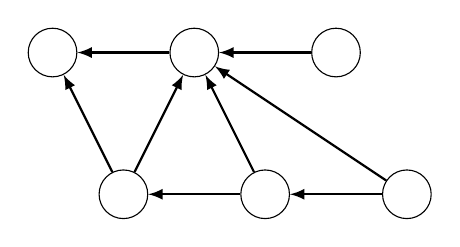
\begin{tikzpicture}[scale=0.9]
\node[draw, circle] (1) at (0,0) {\phantom{0}};
\node[draw, circle] (2) at (2,0) {\phantom{0}};
\node[draw, circle] (3) at (4,0) {\phantom{0}};
\node[draw, circle] (4) at (1,-2) {\phantom{0}};
\node[draw, circle] (5) at (3,-2) {\phantom{0}};
\node[draw, circle] (6) at (5,-2) {\phantom{0}};

\path[draw,thick,->,>=latex] (2) -- (1);
\path[draw,thick,->,>=latex] (3) -- (2);
\path[draw,thick,->,>=latex] (5) -- (4);
\path[draw,thick,->,>=latex] (6) -- (5);
\path[draw,thick,->,>=latex] (4) -- (1);
\path[draw,thick,->,>=latex] (4) -- (2);
\path[draw,thick,->,>=latex] (5) -- (2);
\path[draw,thick,->,>=latex] (6) -- (2);
\end{tikzpicture}
\end{center}
Grundy-luvut ovat seuraavat:
\begin{center}
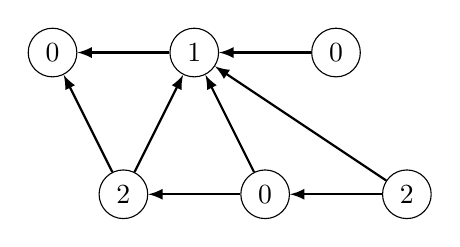
\begin{tikzpicture}[scale=0.9]
\node[draw, circle] (1) at (0,0) {0};
\node[draw, circle] (2) at (2,0) {1};
\node[draw, circle] (3) at (4,0) {0};
\node[draw, circle] (4) at (1,-2) {2};
\node[draw, circle] (5) at (3,-2) {0};
\node[draw, circle] (6) at (5,-2) {2};

\path[draw,thick,->,>=latex] (2) -- (1);
\path[draw,thick,->,>=latex] (3) -- (2);
\path[draw,thick,->,>=latex] (5) -- (4);
\path[draw,thick,->,>=latex] (6) -- (5);
\path[draw,thick,->,>=latex] (4) -- (1);
\path[draw,thick,->,>=latex] (4) -- (2);
\path[draw,thick,->,>=latex] (5) -- (2);
\path[draw,thick,->,>=latex] (6) -- (2);
\end{tikzpicture}
\end{center}
Jos tila on häviötila, sen Grundy-luku on 0.
Jos taas tila on voittotila, sen Grundy-luku
on jokin positiivinen luku.

Grundy-luvun hyötynä on,
että se vastaa tikkujen määrää nim-kasassa.
Jos Grundy-luku on 0, niin tilasta pääsee vain tiloihin,
joiden Grundy-luku ei ole 0.
Jos taas Grundy-luku on $x>0$, niin tilasta pääsee tiloihin,
joiden Grundy-luvut kattavat välin $0,1,\ldots,x-1$.

~\\
\noindent
Tarkastellaan esimerkkinä peliä,
jossa pelaajat siirtävät vuorotellen
pelihahmoa sokkelossa.
Jokainen sokkelon ruutu on lattiaa tai seinää.
Kullakin siirrolla hahmon tulee liikkua jokin
määrä askeleita vasemmalle tai jokin
määrä askeleita ylöspäin.
Pelin voittaja on se, joka tekee viimeisen siirron.

\begin{samepage}
Esimerkiksi seuraavassa on pelin mahdollinen aloitustilanne,
jossa @ on pelihahmo ja * merkitsee ruutua, johon hahmo voi siirtyä.

\begin{center}
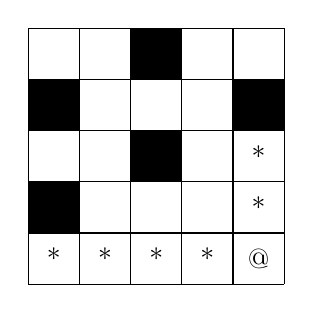
\begin{tikzpicture}[scale=.65]
  \begin{scope}
    \fill [color=black] (0, 1) rectangle (1, 2);
    \fill [color=black] (0, 3) rectangle (1, 4);
    \fill [color=black] (2, 2) rectangle (3, 3);
    \fill [color=black] (2, 4) rectangle (3, 5);
    \fill [color=black] (4, 3) rectangle (5, 4);

    \draw (0, 0) grid (5, 5);
    
    \node at (4.5,0.5) {@};
    \node at (3.5,0.5) {*};
    \node at (2.5,0.5) {*};
    \node at (1.5,0.5) {*};
    \node at (0.5,0.5) {*};
    \node at (4.5,1.5) {*};
    \node at (4.5,2.5) {*};
    
  \end{scope}
\end{tikzpicture}
\end{center}
\end{samepage}

Sokkelopelin tiloja ovat kaikki sokkelon
lattiaruudut. Tässä tapauksessa
tilojen Grundy-luvut ovat seuraavat:

\begin{center}
\begin{tikzpicture}[scale=.65]
  \begin{scope}
    \fill [color=black] (0, 1) rectangle (1, 2);
    \fill [color=black] (0, 3) rectangle (1, 4);
    \fill [color=black] (2, 2) rectangle (3, 3);
    \fill [color=black] (2, 4) rectangle (3, 5);
    \fill [color=black] (4, 3) rectangle (5, 4);

    \draw (0, 0) grid (5, 5);
    

    \setcounter{row}{5}
    \setrow {0}{1}{}{0}{1}
    \setrow {}{0}{1}{2}{}
    \setrow {0}{2}{}{1}{0}
    \setrow {}{3}{0}{4}{1}
    \setrow {0}{4}{1}{3}{2}
    
  \end{scope}
\end{tikzpicture}
\end{center}

Tämän seurauksena sokkelopelin
tila käyttäytyy
samalla tavalla kuin nim-pelin kasa.
Esimerkiksi oikean alakulman ruudun
Grundy-luku on 2,
joten kyseessä on voittotila.
Voittoon johtava siirto on joko liikkua neljä
askelta vasemmalle tai kaksi askelta ylöspäin.

Huomaa, että toisin kuin nim-pelissä,
tilasta saattaa päästä toiseen tilaan,
jonka Grundy-luku on suurempi.
Tällaisen siirron voi kuitenkin
aina peruuttaa niin,
että Grundy-luku palautuu samaksi.

\subsubsection{Alipelit}

Oletetaan seuraavaksi, että peli muodostuu
alipeleistä ja jokaisella vuorolla
pelaaja valitsee jonkin alipeleistä ja
tekee siirron siinä.
Peli päättyy, kun missään alipelissä ei
pysty tekemään siirtoa.

Nyt pelin tilan Grundy-luku on alipelien
Grundy-lukujen nim-summa.
Peliä pystyy pelaamaan nim-pelin
tapaan selvittämällä kaikkien alipelien Grundy-luvut
ja laskemalla niiden nim-summa.

~\\
\noindent
Tarkastellaan esimerkkinä kolmen sokkelon peliä.
Tässä pelissä pelaaja valitsee joka siirrolla
yhden sokkeloista ja siirtää siinä olevaa hahmoa.
Pelin aloitustilanne voi olla seuraavanlainen:

\begin{center}
\begin{tabular}{ccc}
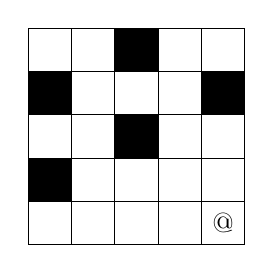
\begin{tikzpicture}[scale=.55]
  \begin{scope}
    \fill [color=black] (0, 1) rectangle (1, 2);
    \fill [color=black] (0, 3) rectangle (1, 4);
    \fill [color=black] (2, 2) rectangle (3, 3);
    \fill [color=black] (2, 4) rectangle (3, 5);
    \fill [color=black] (4, 3) rectangle (5, 4);

    \draw (0, 0) grid (5, 5);

    \node at (4.5,0.5) {@};

    \end{scope}
\end{tikzpicture}
&
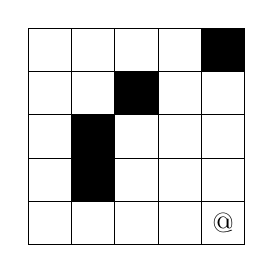
\begin{tikzpicture}[scale=.55]
  \begin{scope}
    \fill [color=black] (1, 1) rectangle (2, 3);
    \fill [color=black] (2, 3) rectangle (3, 4);
    \fill [color=black] (4, 4) rectangle (5, 5);

    \draw (0, 0) grid (5, 5);
    
    \node at (4.5,0.5) {@};

  \end{scope}
\end{tikzpicture}
&
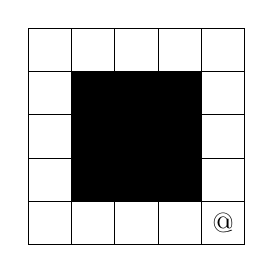
\begin{tikzpicture}[scale=.55]
  \begin{scope}
    \fill [color=black] (1, 1) rectangle (4, 4);

    \draw (0, 0) grid (5, 5);
    
    \node at (4.5,0.5) {@};
  \end{scope}
\end{tikzpicture}
\end{tabular}
\end{center}

Sokkeloiden ruutujen Grundy-luvut ovat:

\begin{center}
\begin{tabular}{ccc}
\begin{tikzpicture}[scale=.55]
  \begin{scope}
    \fill [color=black] (0, 1) rectangle (1, 2);
    \fill [color=black] (0, 3) rectangle (1, 4);
    \fill [color=black] (2, 2) rectangle (3, 3);
    \fill [color=black] (2, 4) rectangle (3, 5);
    \fill [color=black] (4, 3) rectangle (5, 4);

    \draw (0, 0) grid (5, 5);

    \setcounter{row}{5}
    \setrow {0}{1}{}{0}{1}
    \setrow {}{0}{1}{2}{}
    \setrow {0}{2}{}{1}{0}
    \setrow {}{3}{0}{4}{1}
    \setrow {0}{4}{1}{3}{2}

    \end{scope}
\end{tikzpicture}
&
\begin{tikzpicture}[scale=.55]
  \begin{scope}
    \fill [color=black] (1, 1) rectangle (2, 3);
    \fill [color=black] (2, 3) rectangle (3, 4);
    \fill [color=black] (4, 4) rectangle (5, 5);

    \draw (0, 0) grid (5, 5);

    \setcounter{row}{5}
    \setrow {0}{1}{2}{3}{}
    \setrow {1}{0}{}{0}{1}
    \setrow {2}{}{0}{1}{2}
    \setrow {3}{}{1}{2}{0}
    \setrow {4}{0}{2}{5}{3}    
    
  \end{scope}
\end{tikzpicture}
&
\begin{tikzpicture}[scale=.55]
  \begin{scope}
    \fill [color=black] (1, 1) rectangle (4, 4);

    \draw (0, 0) grid (5, 5);

    \setcounter{row}{5}
    \setrow {0}{1}{2}{3}{4}
    \setrow {1}{}{}{}{0}
    \setrow {2}{}{}{}{1}
    \setrow {3}{}{}{}{2}
    \setrow {4}{0}{1}{2}{3}    
    
  \end{scope}
\end{tikzpicture}
\end{tabular}
\end{center}

Aloitustilanteessa Grundy-lukujen nim-summa on
$2 \oplus 3 \oplus 3 = 2$, joten
aloittaja pystyy voittamaan pelin.
Voittoon johtava siirto on liikkua vasemmassa sokkelossa
2 askelta ylöspäin, jolloin nim-summaksi
tulee $0 \oplus 3 \oplus 3 = 0$.

\subsubsection{Jakautuminen}

Joskus siirto pelissä jakaa pelin alipeleihin,
jotka ovat toisistaan riippumattomia.
Tällöin pelin Grundy-luku on

\[\textrm{mex}(\{g_1, g_2, \ldots, g_n \}),\]
missä $n$ on siirtojen määrä ja
\[g_k = a_{k,1} \oplus a_{k,2} \oplus \ldots \oplus a_{k,m},\]
missä siirron $k$ tuottamien alipelien
Grundy-luvut ovat $a_{k,1},a_{k,2},\ldots,a_{k,m}$.

\index{Grundyn peli}

Esimerkki tällaisesta pelistä on \key{Grundyn peli}.
Pelin alkutilanteessa on kasa, jossa on $n$ tikkua.
Joka vuorolla pelaaja valitsee jonkin kasan
ja jakaa sen kahdeksi epätyhjäksi kasaksi
niin, että kasoissa on eri määrä tikkuja.
Pelin voittaja on se, joka tekee viimeisen jaon.

Merkitään $f(n)$ Grundy-lukua kasalle,
jossa on $n$ tikkua.
Grundy-luku muodostuu käymällä läpi tavat
jakaa kasa kahdeksi kasaksi.
Esimerkiksi tapauksessa $n=8$ mahdolliset jakotavat
ovat $1+7$, $2+6$ ja $3+5$, joten
\[f(8)=\textrm{mex}(\{f(1) \oplus f(7), f(2) \oplus f(6), f(3) \oplus f(5)\}).\]
Tässä pelissä luvun $f(n)$ laskeminen vaatii lukujen
$f(1),\ldots,f(n-1)$ laskemista.
Pohjatapauksina $f(1)=f(2)=0$, koska 1 ja 2 tikun
kasaa ei ole mahdollista jakaa mitenkään.
Ensimmäiset Grundy-luvut ovat:
\[
\begin{array}{lcl}
f(1) & = & 0 \\
f(2) & = & 0 \\
f(3) & = & 1 \\
f(4) & = & 0 \\
f(5) & = & 2 \\
f(6) & = & 1 \\
f(7) & = & 0 \\
f(8) & = & 2 \\
\end{array}
\]
Tapauksen $n=8$ Grundy-luku on 2, joten peli on mahdollista
voittaa.
Voittosiirto on muodostaa kasat $1+7$,
koska $f(1) \oplus f(7) = 0$.